% THIS IS SIGPROC-SP.TEX - VERSION 3.1
% WORKS WITH V3.2SP OF ACM_PROC_ARTICLE-SP.CLS
% APRIL 2009
%
% It is an example file showing how to use the 'acm_proc_article-sp.cls' V3.2SP
% LaTeX2e document class file for Conference Proceedings submissions.
% ----------------------------------------------------------------------------------------------------------------
% This .tex file (and associated .cls V3.2SP) *DOES NOT* produce:
%       1) The Permission Statement
%       2) The Conference (location) Info information
%       3) The Copyright Line with ACM data
%       4) Page numbering
% ---------------------------------------------------------------------------------------------------------------
% It is an example which *does* use the .bib file (from which the .bbl file
% is produced).
% REMEMBER HOWEVER: After having produced the .bbl file,
% and prior to final submission,
% you need to 'insert'  your .bbl file into your source .tex file so as to provide
% ONE 'self-contained' source file.
%
% Questions regarding SIGS should be sent to
% Adrienne Griscti ---> griscti@acm.org
%
% Questions/suggestions regarding the guidelines, .tex and .cls files, etc. to
% Gerald Murray ---> murray@hq.acm.org
%
% For tracking purposes - this is V3.1SP - APRIL 2009

\documentclass{acm_proc_article-sp}
%\documentclass{sig-alternate}
\usepackage[numbers, sort, compress]{natbib}
\usepackage{xspace}
\usepackage{color}
%\usepackage{hyperref}
%\usepackage{mdwlist}
\usepackage{url}
\usepackage{subfigure}
%\usepackage{hyphenation}
\hyphenation{Map-Reduce}
\usepackage{listings} 
\usepackage{enumerate}

\newif\ifdraft
\drafttrue

\ifdraft
\newcommand{\terminology}[1]{ {\textcolor{red} {(Terminology used: \textbf{#1}) }}}
\newcommand{\jhanote}[1]{ {\textcolor{red} { ***shantenu: #1 }}}
\newcommand{\alnote}[1]{ {\textcolor{blue} { ***andreL: #1 }}}
\newcommand{\pnote}[1]{ {\textcolor{magenta} { ***pradeep: #1 }}}
\newcommand{\note}[1]{ {\textcolor{red} { ***Note: #1 }}}
\else
\newcommand{\terminology}[1]{}
\newcommand{\alnote}[1]{}
\newcommand{\pnote}[1]{}
\newcommand{\jhanote}[1]{}
\newcommand{\note}[1]{}
\fi



\newcommand{\pilot}{Pilot\xspace}
\newcommand{\pilots}{Pilots\xspace}
\newcommand{\pilotjob}{Pilot-Job\xspace}
\newcommand{\pilotjobs}{Pilot-Jobs\xspace}
\newcommand{\pilotmapreduce}{Pilot-MapReduce\xspace}
\newcommand{\computeunit}{Compute Unit\xspace}
\newcommand{\computeunits}{Compute Units\xspace}
\newcommand{\cu}{CU\xspace}
\newcommand{\cus}{CUs\xspace}
\newcommand{\cs}{Compute Service\xspace}
\newcommand{\css}{Compute Services\xspace}
\newcommand{\pcs}{Pilot Compute Service\xspace}
\newcommand{\dataunit}{Data Unit\xspace}
\newcommand{\dataunits}{Data Unit\xspace}
\newcommand{\du}{DU\xspace}
\newcommand{\dus}{DUs\xspace}
\newcommand{\pilotdata}{Pilot-Data\xspace}
\newcommand{\pd}{PD\xspace}
\newcommand{\pds}{Pilot Data Service\xspace}
\newcommand{\pdss}{Pilot Data Services\xspace}
\newcommand{\su}{SU\xspace}
\newcommand{\sus}{SUs\xspace}
\newcommand{\schedulableunit}{Schedulable Unit\xspace}
\newcommand{\schedulableunits}{Schedulable Units\xspace}
\begin{document}

%\title{An Extensible Pilot-based MapReduce Implementation}
\title{Pilot-MapReduce: An Extensible and Flexible
  MapReduce Implementation for Distributed Data}

%
% You need the command \numberofauthors to handle the 'placement
% and alignment' of the authors beneath the title.
%
% For aesthetic reasons, we recommend 'three authors at a time'
% i.e. three 'name/affiliation blocks' be placed beneath the title.
%
% NOTE: You are NOT restricted in how many 'rows' of
% "name/affiliations" may appear. We just ask that you restrict
% the number of 'columns' to three.
%
% Because of the available 'opening page real-estate'
% we ask you to refrain from putting more than six authors
% (two rows with three columns) beneath the article title.
% More than six makes the first-page appear very cluttered indeed.
%
% Use the \alignauthor commands to handle the names
% and affiliations for an 'aesthetic maximum' of six authors.
% Add names, affiliations, addresses for
% the seventh etc. author(s) as the argument for the
% \additionalauthors command.
% These 'additional authors' will be output/set for you
% without further effort on your part as the last section in
% the body of your article BEFORE References or any Appendices.

\numberofauthors{3} %  in this sample file, there are a *total*
% of EIGHT authors. SIX appear on the 'first-page' (for formatting
% reasons) and the remaining two appear in the \additionalauthors section.
%
\author{
% You can go ahead and credit any number of authors here,
% e.g. one 'row of three' or two rows (consisting of one row of three
% and a second row of one, two or three).
%
% The command \alignauthor (no curly braces needed) should
% precede each author name, affiliation/snail-mail address and
% e-mail address. Additionally, tag each line of
% affiliation/address with \affaddr, and tag the
% e-mail address with \email.
%
\alignauthor Pradeep Kumar Mantha\\
       \affaddr{Center for Computation and Technology}\\
       \affaddr{Louisiana State University}\\
       \affaddr{216 Johnston}\\
       \affaddr{Baton Rouge, LA}
       \email{pmanth2@cct.lsu.edu}
\alignauthor Andre Luckow\\
       \affaddr{Center for Computation and Technology}\\
       \affaddr{Louisiana State University}\\
       \affaddr{216 Johnston}\\
       \affaddr{Baton Rouge, LA}
       \email{aluckow@cct.lsu.edu} 
\alignauthor Shantenu Jha\titlenote{Author for correspondence}\\
      \affaddr{Center for Autonomic Computing}\\
     \affaddr{Rutgers University}\\
      \affaddr{94 Brett Road}\\
      \affaddr{Piscataway, NJ}
     \email{shantenu.jha@rutgers.edu}
}
% There's nothing stopping you putting the seventh, eighth, etc.
% author on the opening page (as the 'third row') but we ask,
% for aesthetic reasons that you place these 'additional authors'
% in the \additional authors block, viz.
% \additionalauthors{Additional authors: John Smith (The Th{\o}rv{\"a}ld Group,
% email: {\texttt{jsmith@affiliation.org}}) and Julius P.~Kumquat
% (The Kumquat Consortium, email: {\texttt{jpkumquat@consortium.net}}).}
\date{30 July 1999}
% Just remember to make sure that the TOTAL number of authors
% is the number that will appear on the first page PLUS the
% number that will appear in the \additionalauthors section.

\maketitle
\begin{abstract}
  The volume and complexity of data that must be analyzed is
  increasing exponentially.  Inevitably, the ability to analyze data
  by localizing it will yield limited returns; additionally, this data
  is naturally distributed; Thus, efficient processing of large
  distributed datasets are required, whilst yet not introducing
  fundamentally new programming models or methods. For example,
  MapReduce is a proven effective programming model for processing
  large datasets.  There are reasons to assume that with an effective
  and efficient runtime environment it will be effective with
  distributed data too, without refactoring MapReduce itself. The
  effectiveness of MapReduce on distributed data depends on effective
  distributed coordination of computation (map and reduce) and data,
  as well as distributed data management (in particular the transfer
  of intermediate data units).  To address these requirements, we
  design and implement \pilotmapreduce (PMR) -- a flexible,
  infrastructure-indepen\-dent runtime environment for MapReduce-based
  applications. PMR is based on \pilot abstractions for both compute
  (Pilot-Jobs) and data (Pilot-Data): it utilizes Pilot-Jobs to couple
  the map phase computation to the nearby source data, and Pilot-Data
  to move intermediate data using parallel data transfers to the
  reduce computation phase.  We show the effectiveness of PMR using
  different applications with different characteristics (e.\,g.\
  different volumes of intermediate and output data). Our experimental
  evaluations show that the Pilot abstraction for data movement across
  multiple clusters is promising, and can %provide % minimizes overall
  lower the execution time span of the entire MapReduce execution. We
  also investigate the scalability of PMR across multiple clusters by
  comparing it with SEQAL which is a Hadoop based MapReduce
  application.
% We analyze the effectiveness of PMR for
% different applications based upon the ratio of data-aggregation between phases
% as well as single and hierarchical MapReduce.
\end{abstract}

%Hierarchical MapReduce is a potential distributed solution only for
%high data aggregation applications leaving single cluster-MapReduce as
%an optimal solution for zero or ballooning data applications~\cite
%{weissman-mr-11}, which is still costly as it involves initial huge
%data transfers of source data to the single cluster.

% A category with the (minimum) three required fields
\category{D.1.2}{Software}{MapReduce}
%A category including the fourth, optional field follows...
\category{J.3}{Computer Applications}{Bioinformatics, Mapping}

% \terms{Design, Experimentation, Performance}

\keywords{Pilot-Jobs, Data-Intensive, MapReduce, Genome Sequencing, BWA,  Distributed Computing}% NOT required for Proceedings

\section{Introduction}

%General Motivation

There are various challenges associated with processing of data at
extreme scales: which has become a critical factor in many science
disciplines, e.\,g.\ in the areas of fusion energy (ITER),
bioinformatics (metagenomics), climate (Earth System Grid), and
astronomy
(LSST)~\cite{Berriman:2011:AAS:2039359.2047483,Jha:2011fk}. The
volumes of data produced by these scientific applications is
increasing rapidly, driven by advanced technologies (e.\,g.\
increasing compute capacity and higher resolution sensors) and
decreasing costs for computation, data acquisition and
storage~\cite{hey2009}. The number of scientific applications that
either currently utilize, or need to utilize large volumes of
potentially distributed data is immense. The challenges faced by these
applications are interoperability, efficiently managing compute tasks,
and moving data to the scheduled compute location.

% which is inevitable in case of programming models like MapReduce.

%Intro to MapReduce
Processing large volumes of data is a challenging task. MapReduce is
an effective programming model for addressing this challenge.
MapReduce~\cite{Dean:2004:MSD:1251254.1251264} as originally developed
by Google aims to address the big data problem by providing an
easy-to-use abstraction for parallel data processing. The most
prominent framework for doing MapReduce computations is Apache
Hadoop~\cite{hadoop}. However, there are limitations to the current MR
implementations: (i) They lack a modular architecture, (ii) are
tied to specific infrastructure, e.\,g.\ Hadoop relies on the Hadoop
File System (HDFS), and (iii) do not provide efficient support for
dynamic and processing distributed data, e.\,g.\ Hadoop is designed
for cluster/local environment, but not for a high degree of
distribution.

% In particular when the source
% data and computing platform distributed widely, the most efficient
% architecture for processing data over the entire data set becomes non-trivial.
%Intro to weissman's MapReduce configurations and workload types.
%Why pilot abstractions

% as well as the limitations of existing MapReduce implementations, such
% as the limited support for distributed data. 

Pilot abstractions enable the clean separation of resource management
concerns and application/frameworks. In particular, \pilotjobs have
been notable in their ability to manage large numbers of compute units
across multiple high performance clusters, providing decoupling
application-level scheduling and system-level resource
management. But, there is also a need of an abstraction to liberate
applications from the challenging task of compute-data placement and
scheduling. The Pilot-API~\cite{pstar-2012} aims to address this issue
by providing a unified API for managing both compute and data
pilots. In this paper, we present \emph{BigData (BD)}, an extension of
the BigJob framework (BJ)~\cite{bigjob_web} to data. Both BigJob and
BigData provide a full implementation of the Pilot-API and enable the
management of resources, compute \& data units as well as the
relationships between them. Specifically, the Pilot-API promotes
affinities as a first class characteristic for describing such
relationships between compute and data elements and to support dynamic
decision making. 

% Pilot-Data provides an abstraction
% for expressing and managing relationships between data units and/or compute
% units. The coupling of abstractions, Pilot-Jobs and Pilot-Data, provide a
% complete solution for data intensive applications to utilize distributed cyber
% infrastructure effectively. 

A critical aspect of MapReduce, is the management of data and compute
localities as well as the management of data movements, e.\,g.\
between the map and the reduce phase.  In this paper, we demonstrate
the efficient support of these capabilities via the Pilot
abstractions. We design and implement \pilotmapreduce \ -- a novel
\pilot-based MapReduce implementation which enables clean separation
of resource management and MapReduce application. We show how \pilot
abstractions are used for managing the map and reduce tasks and
intermediate shuffle data between them.  In addition, we show the
advantages of the \pilot-based architecture in terms of flexibility,
extensibility, scalability and performance; for example, we discuss
the usability of \pilot-abstractions in designing dynamic execution
workflows which involves multiple MapReduce computations.

\pnote{The key take-aways of this paper are:
\begin{itemize}
	\item MapReduce simplifies the construction of data-parallel applications.
	\item Pilot-Abstraction enable the clean separation of resource management concerns and MapReduce.
	\item The Pilot/SAGA-based approach enables a maximum of portability, interoperability and code-reuse.
	\item Hadoop is designed for cluster/local environment, but not for a high degree of distribution.
	\item Future work: dynamic execution.
\end{itemize}  - repetitive? }

Before we proceed further, it is critical to emphasize that it is not
the aim of this paper to suggest PMR as a replacement to Hadoop.
However, we posit that where MR-based applications need to be employed
over distributed data, including but not limited to clusters connected
over WAN, or production distributed cyberinfrastructure such as XSEDE,
EGI, PMR provides a flexible, extensible implementation of MR that is
also efficient.
 

This paper is organized as follows: Section~\ref{sec:related_work} presents
related works. Section~\ref{sec-pilot-impl} gives an overview of \pilot
abstractions and the BigData framework. In section~\ref{sec-pilot-mr} we discuss
the design and implementation of the \pilotmapreduce framework.
Section~\ref{sec-experiments} gives experiment setup and result analysis. The
conclusion and future work are given in Section~\ref{sec-conclusion}.


% Introduction must lay out the fact that PMR does not as a
%   substitute Hadoop on dedicated clusters, but is useful on WAN
%   clusters and production infrastructure}

\section{Related and Background Work}
\label{sec:related_work}
The MapReduce programming model~\cite{Dean:2004:MSD:1251254.1251264}
and the distributed file system (Google File System
(GFS)~\cite{Ghemawat:2003:GFS:1165389.945450}) it is based on was
originally pioneered by Google. Apache Hadoop~\cite{hadoop} is an open
source implementation of MapReduce. Hadoop also includes an
implementation of a distributed file system -- the Hadoop File System
(HDFS)~\cite{Borthakur:2007fk}. In addition the Hadoop ecosystems
includes several other projects, such as HBase (a system also inspired
by Google's BigTable), Hive, Pig and Zookeeper. The main limitation of
Hadoop MapReduce is that it forces applications into a very rigid
model. Hadoop e.\,g.\ is well suited for running a single MapReduce
application, but very limited in terms of extensibility, e.\,g.\ it
cannot efficiently run an ensemble of MapReduce simulations or support
a pipeline of multiple MapReduce tasks.

Sector/Sphere~\cite{Gu_Grossman_2009} is a parallel data processing framework
consisting of an distributed file system (Sector) and a data processing engine
(Sphere). In contrast to Hadoop, Sphere is able to execute arbitrary 
user-defined function on a stream of data. Hadoop in contrast operates on top 
of file system chunks.

Twister~\cite{Ekanayake:2010:TRI:1851476.1851593} is a 
MapReduce addressing particularly the requirement for supporting iterative 
MapReduce jobs. Twister allows the flexible composition of applications by 
specifying map and reduce tasks and the data flow between these tasks. 

Dryad~\cite{Isard:2007:DDD:1272998.1273005} provides distributed execution of
coarse-grain data-parallel applications. The entire execution is represented in
the form of data flow graphs, where the vertices represent the computational
tasks that can be paralleled on a set of computational resources and the links
between vertices tell Dryad what other vertices need to complete before a
particular vertex can start.

SAGA-MapReduce~\cite{Sehgal:2011:UAI:1945091.1945329} is a SAGA-based
MapReduce implementation that utilizes the SAGA-API for accessing system-level
features, such as resource management, file management and coordination. The
SAGA-based approach enabled the decoupling of infrastructure and application
concerns enabling the support of a wide-set of distributed infrastructure
(e.\,g,\ grids and clouds). The utilization of Pilot abstractions has several
advantages compared to the SAGA-only approach: (i) compute and data pilots
allow an efficient decoupling of resource allocation and usage, i.\,e.\ the
MapReduce master can efficiently schedule compute units containing mapper and
reduce tasks; (ii) the co-location of data and compute units descriptively
defined and are automatically handled by Pilot framework; This enables the
applications to easily trade-off data transfers and available compute
capacities.


In this paper, we discuss usability of \pilot-abstractions to design a flexible, 
infrastructure-independent runtime environment for MapReduce application. In 
contrast to previous approaches \pilotmapreduce heavily relies on \pilot 
abstractions for de-coupling the MapReduce runtime, application-level scheduling 
and resource management providing a high degree of flexibility and extensibility.



%data flow oriented frameworks

% Twitter Storm - \pnote{ Andre- Could you please add information about twitter storm}


\section{Pilot Abstractions}
\label{sec-pilot-impl}

Pilot-abstractions provide effective management of compute and data units and the relationships between them(affinities).  They liberate 
the applications from the challenging  requirement of assigning/scheduling the compute or data unit onto a particular resource.

\subsection{Pilot Abstractions for Compute}
The abstraction of a {\emph \pilotjob} (PJ) generalizes the reoccurring concept of
utilizing a placeholder job as a container for a set of compute tasks;
instances of that placeholder job are commonly referred to as Pilot-Jobs or
pilots. The PJ provides applications (user) level control and management of
the set of allocated resources. 

BigJob (BJ) is a SAGA-based PJ framework. BJ has been designed to be general-purpose and extensible. 
While BJ has been originally built for HPC infrastructures, such as XSEDE and FutureGrid, it is generally also usable in other environments. 
This extensibility mainly arises from the usage of SAGA as a common API for accessing distributed resources. 
SAGA provides a simple, POSIX-style API to the most common grid functions at a sufficiently high-level of abstraction 
so as to be independent of the diverse and dynamic grid environments.~\cite{pstar-2012}

\subsection{Pilot Abstractions for Data}
Analogous to \pilotjobs, {\emph Pilot-Data}(PD)
provides late-binding capabilities for data by separating the allocation of
physical storage and application-level data units~\cite{pstar-2012}.

\begin{figure}[htbp]
	\centering
		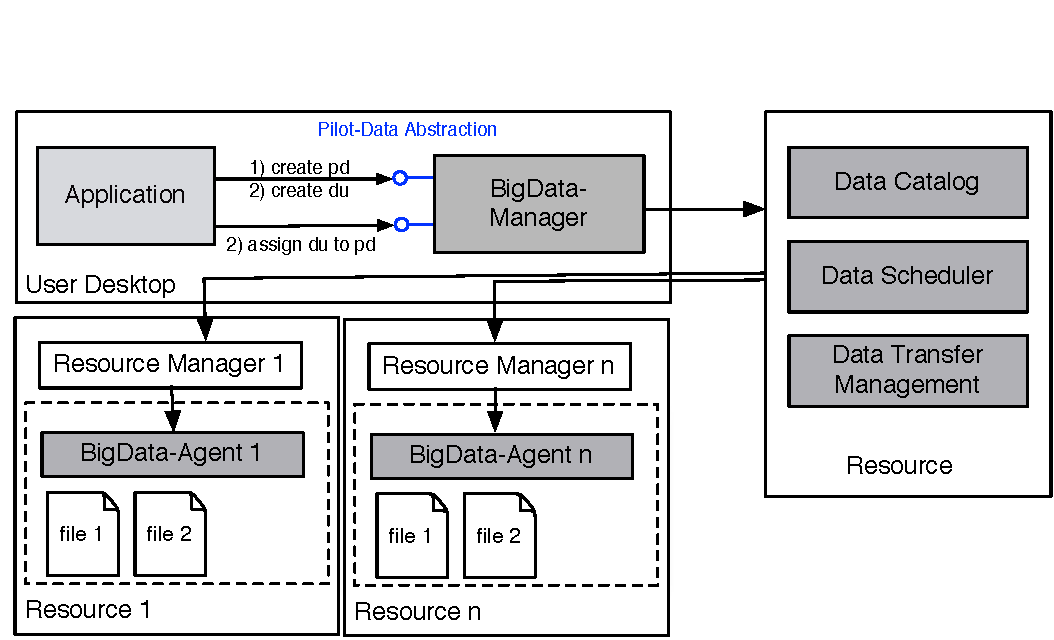
\includegraphics[width=0.47\textwidth]{figures/bigdata.pdf}
	\caption{BigData Architecture and Interactions}
	\label{fig:figures_bigdata}
\end{figure}

{\it BigData (BD)} is an implementation of the Pilot-Data abstraction. BigData
is designed to work together with \emph{BigJob (BJ)}~\cite{bigjob_web} -- a
SAGA-based Pilot-Job implementation. Figure~\ref{fig:figures_bigdata} gives an
overview of the architecture. The system consists similarly to BigJob of two
components: the BD-Manager and the BD-Agents deployed on the physical resources.
The coordination scheme used is again M/W with some intelligence that is located
de-centrally at the BD-Agent. As communication mechanism the SAGA Advert Service
is used, in a similar push/pull mode as for BJ.

The BD-Manager is responsible for (i) meta-data management, i.\,e.\ it
keeps track of the pilot stores that a pilot data object is associated
with, (ii) for scheduling data movements and data replications (taking
into account the application requirements defined via affinities), and
(iii) for managing data movements activities. For this purpose, it can rely
on external service, e.\,g.\ Globus Online for data transfer management.  
Similar to BigJob, an agent on each resource is used to manage the physical 
storage on a resource.  

A particular critical requirement for data-intensive application, is
the management of affinity between CUs and also between DUs and
DUs. The BD scheduler supports preliminary affinity-aware
scheduling: both BigJob and BigData are tightly integrated to
efficiently support compute- and data-related aspects of dynamic
execution. 

\subsection{Pilot-API and Affinities}
\label{sec-affinities}

The Pilot-API is an {\it interoperable} and {\it extensible} API which exposes the core functionalities
of a \pilot framework via a unified interface providing a common API that can be used across multiple 
distinct production cyber infrastructures.
 The API provides three core classes: the
\texttt{PilotComputeService} for the management of Pilot-Jobs,
\texttt{PilotDataService} for the management of Pilot-Data and the
\texttt{ComputeDataService} for the management of \texttt{ComputeUnits} (CUs)
and \texttt{DataUnits} (DUs). A CU represents a primary self-containing piece
of work, while a DU represents a logical set for data~\cite{pstar-2012}.

% \subsection{Affinities}

The Pilot-API promotes \emph{affinities} as a first class characteristic for
describing relationships between data and/or compute supporting dynamic decision
making. Unfortunately, most production infrastructure lack system-level support
for affinities, e.\,g.\ resource localities cannot be introspected. Data storage
in particular in distributed settings, such as in the XSEDE or the EGI
environment, is often a black box for the application with unknown quality of
services, i. e. the application usually does not know what bandwidths and
latencies it can expect. To address these deficiency the Pilot-API introduces 
affinities on application-level: applications can associate compute and data 
units as well as resources  (the \pilots) with affinity labels. The BigJob and 
BigData runtime will then ensure that CUs and DUs are placed with respect to the 
affinity requirements of the application.


\section{Pilot-MapReduce -- A Pilot-based MapReduce Implementation}
\label{sec-pilot-mr}
%\alnote{We should only use PilotMapReduce to refer to our framework - SAGA does not need to be in the name and mentioned all the time}

\jhanote{Not sure why we have the first instanc of ``\pilotmapreduce''
  in ``\emph''. Also we toggle between PMR and
  ``\pilotmapreduce''. Please be consistent} \alnote{ok removed emph}
  

\pilotmapreduce (PMR) is a \pilot-based implementation of the
MapReduce programming model. PMR decouples the core MapReduce
framework from the actual management of the compute, data and network
resources. By decoupling job scheduling and monitoring from the
resource management, PMR can efficiently re-use the resource
management and late-binding capabilities of BigJob and BigData. PMR
exposes an easy-to-use interface (Pilot-API) which provides the
\jhanote{Need to talk about the following sentence/claim...} complete
functionality needed by any MapReduce algorithm, while hiding the more
complex functionality, such as chunking of the input, sorting the
intermediate results, managing and coordinating the map \& reduce
tasks, etc., these are generically implemented by the framework.



%\alnote{Can we put a code snipped in here somewhere? maybe a separate sub-section}

%Pilot-API is used for managing map and reduce compute units
%and for defining relationships between the intermediate data and reduce tasks
%across distributed infrastructure


\subsection{Architecture of \pilotmapreduce}
\pilotmapreduce introduces a clean separation of concerns between
compute and data management on the one hand, with their scheduling in
a distributed context. The pilot abstraction enable the easy
acquisition of both compute and storage resources. The MR manager can
focus on orchestrating this resource pool. This architecture can also
efficiently support workloads that currently cannot be support well
enough by Hadoop, e.\,g.\ iterative
applications. Figure~\ref{fig:figures_mapreduce-pilotdata} shows the
architecture of the \pilotmapreduce framework.

\begin{figure}[htbp]
	\centering
	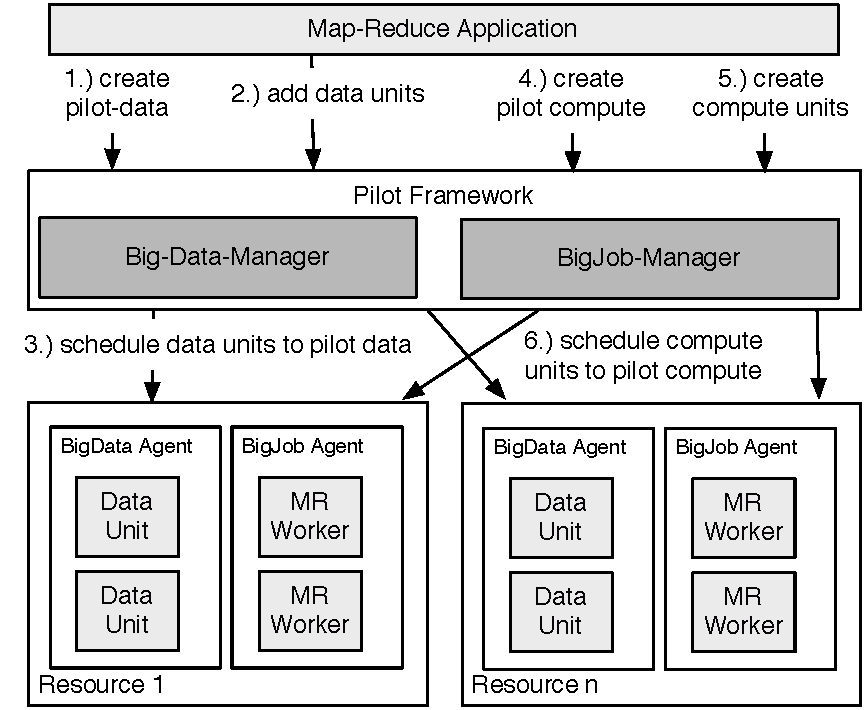
\includegraphics[width=0.4\textwidth]{figures/mapreduce-pilotdata.pdf}
	\caption{\textbf{Pilot-based MapReduce:} Each pilot (both compute and data 
	pilot) can be associated with an affinity label. The BigData and BigJob 
	Manager will ensure that CUs and DUs are placed with respect to these 
	requirements.}
	\label{fig:figures_mapreduce-pilotdata}
\end{figure}

The flow of a typical MapReduce application involves the chunking of
the data, the execution of the map compute tasks, shuffling and moving
the intermediate data to the reduce task and finally the execution of
the reduce tasks.  \pilotmapreduce utilizes a set of compute and data
pilots for this application workflow: % \jhanote{Worth noting that
%   these numbers don't correspond to the numbers in Figure 2, which in
%   of itself is not a problem, but we should try to make sure the
%   reader doesn't look to figure 2 to understand these
%   steps..}\alnote{changed enumeration list to A., B. referencing steps
%   in fig.}
\begin{enumerate}[A.]
\item Initially, the MR manager allocates a set of compute and data
  resources by starting one (or most often a set of) compute and data
  pilots on different resources (step 1 and 2 in
  figure~\ref{fig:figures_mapreduce-pilotdata}). In general, on each
  resource one compute and one data pilot is co-located. The data
  pilot is either created with reference to local input data or the
  input data is moved to the data pilot after its creation.

\item \textbf{Chunking:} The input data is {\it chunked}. BigJob is
  used as general abstraction for executing CUs. Thus, the MR-Manager
  executes a set of chunk compute units via BJ. The execution of
  the chunk CUs is captured in step 5 and 6 in
  figure~\ref{fig:figures_mapreduce-pilotdata}. \label{stp:chunking}
	
\item \textbf{Mapping:} The frameworks assigned a set of {\it map} CUs
  to the chunks created in step~\ref{stp:chunking}. Again, BJ is used
  for managing the CUs. BJ and BD ensures that CUs and DUs are
  co-located. The execution of the map CUs is done analogous to the
  chunk CUs (step 5/6).
	
\item \textbf{Shuffling:} %\pnote{partitioning and sorting of
  % map output is part of map task}. \alnote{Hadoop Definitive Guide:
  % ``The process by which the system performs the sort and transfers
  % the map outputs to the reducers as inputs is known as the
  % shuffle.'' - I would prefer to work with this definition since it
  % encapsulates this intermediate step very well. Rather then
  % including it in the mapping phase (even if it might be done
  % partially by the mapper process.) }

  After the processing is finished the output data is sorted and
  partitioned into multiple DU. Then, data is moved from the map CUs
  to the location of the reduce CUs. For each reduce task a Data Unit
  containing the necessary input files is created and submitted to
  BigData (step 3/4 in figure~\ref{fig:figures_mapreduce-pilotdata})
		
  % \alnote{We need to introduce what we mean by a distributed PMR.}
	
\item \textbf{Reducing:} The {\it reduce} tasks are prepared and
  executed via BJ on the DUs representing the intermediate data (step
  5/6 in figure~\ref{fig:figures_mapreduce-pilotdata}).  The
  management of the data transfers is done by BJ and BD. For this
  purpose, each reduce CU reference a certain DU as dependency.
	
	\item The \pilots are terminated.

\end{enumerate}

\jhanote{The mapping from the Chunking/Mapping/Shuffling stages to the
  diagram steps is a bit hard to grasp. For example although we talk
  about chunking, we find a mention of step 5/6..}

The Pilot-API provides a well-defined abstraction for supporting the
late-binding of compute and data units. The API also allows the
expression and management of relationships between data units and/or
compute units. BigJob and BigData provide an implementation of the
Pilot-API. Both frameworks ensure that the data and compute affinity
requirements of the MapReduce applications are met for each step of
the MapReduce workflow. \jhanote{we don't elaborate how/why.}

\subsection{Compute and Data Management}
The PMR relies on the master/worker coordination model, i.\,e.\ a
central MapReduce-Manager is responsible for coordinating the
MapReduce workers, which in turn are responsible for executing map and
reduce tasks. The MapReduce-Manager utilizes BigJob for executing
mapper and reduce tasks (Listing~\ref{lst:pcs_creation}).

\alnote{Can we do a MR specific example?}

\lstset{
language=Python,
frame=single,
captionpos=b,
stringstyle=\ttfamily,
basicstyle=\scriptsize\ttfamily
}
\noindent\begin{minipage}{0.47 \textwidth}
\begin{lstlisting}[caption={\textbf{Pilot Compute Creation:} Instantiation of a Pilot Job using Pilot Compute Description}, label={lst:pcs_creation}]
pcs = PilotComputeService()
cds = ComputeDataService()
pjd ={"service_url":"pbs-ssh://sierra.futuregrid.org", 
"number_of_processes": '8',
"walltime":10, 
"processes_per_node:'8',
"affinity_datacenter_label":'sierra',
"affinity_machine_label":'sierra'}
pj=pcs.create_pilot(pilot_compute_description=pjd)
cds.add_pilot_compute_service(pcs)
\end{lstlisting}
\end{minipage}

Similarly, Hadoop also utilizes a job and task tracker: the job
tracker is the central manager that dispatches map and reduce tasks to
the nodes of the Hadoop cluster. On each node the task tracker is
responsible for executing the respective tasks. The main limitation of
this architecture is the fact that it intermixes both cluster resource
management and application-level task managements. Thus, it is not
easily possible to integrate Hadoop with another resource management
tool, e.\,g.\ PBS or Torque. Also, the job tracker represents a single
point of failure and scalability bottleneck.

% \subsection{Data Management in \pilotmapreduce}

The efficiency of PMR in particular on multiple resources depends on
the management of the the intermediate data. BigData not only
provides flexibility to manage the relationship between data and
compute units, but also allows {\it parallel} data transfers between
machines and between data units.  BigData is used for moving the
intermediate output files of the mapper tasks to the resource where
the reduce compute units are executed.  Listing~\ref{lst:pds_creation}
illustrates the creation of a new Pilot-Data at the location of the
reduce task.


\alnote{Can we do a MR specific example? Showing the co-placement of compute and 
data}

\lstset{
language=Python,
frame=single,
captionpos=b,
stringstyle=\ttfamily,
basicstyle=\scriptsize\ttfamily
}
\noindent\begin{minipage}{0.47 \textwidth}
\begin{lstlisting}[caption={\textbf{Pilot Data Creation:} Instantiation of a Pilot Data using Pilot Data Description}, label={lst:pds_creation}]
pds = PilotDataService()
pd_desc=
{"service_url":"ssh://india.futuregrid.org/pilotdata",
"size":100,
"affinity_datacenter_label":'india',
"affinity_machine_label":'india'}
pd=pds.create_pilot( pilot_data_description=pd_desc)
cds.add_pilot_data_service(pds)
\end{lstlisting}
\end{minipage}

\alnote{\textbf{removed for now - maybe add later for analysis of perf:} Similarly, Hadoop uses mapred.reduce.parallel.copies parameter to set
the number of parallel transfers run by reduce during the
copy (shuffle) phase.  and use key names for pieces of data which
inform Hadoop how to send related bits of information to a common
destination node.}
%~\footnote{\url{http://developer.yahoo.com/hadoop/tutorial/module1.html}}



\subsection{Distributed MapReduce}
\label{sec:pmr-distributed}
An increasing amount of data that scientific applications need to
operate on is distributed. In many cases the place of data generation
and processing are far apart: For example, the Earth Science Grid
federates data of various climate simulations~\cite{ESG}. Meta-genomic
workflows need to process and analyze data generated by various
sequencing machines~\cite{Jha:2011fk}; the localization onto a single
resource is often not a possibility.

Several options for running Hadoop on distributed data have been
proposed~\cite{weissman-mr-11}: (i) in a global MapReduce setup one
central JobTracker and HDFS NameNode is used for managing a
distributed set of resources; (ii) in a hierarchical MapReduce setup
multiple MapReduce clusters are used: a MapReduce cluster close to the
data source for pre-processing data and a central cluster for
aggregating the different de-central data sources. The volume of the
pre-processed data is generally lower and thus, can be easily moved to
another processing resource. 

Weissman et.\,al~\cite{weissman-mr-11} show that a hierarchical Hadoop
configuration leads to a better performance than a naive global Hadoop
cluster for some application. A main drawback of this approach is the
increased complexity: Hadoop is not designed with respect to a
federation of multiple MapReduce clusters. Thus, setting up such a
system requires a lot of manual effort. 

\pilotmapreduce in contrast provides an abstraction of unified compute
and data resources; thus MapReduce framework can be used to reason
about data and compute localities and is able to operate on a dynamic
and distributed pool of storage and compute resources.  BigJob and
BigData will ensure that the affinity requirements of the MR framework
are met. \jhanote{The last sentence is a repitition}

\begin{figure}
	\centering
	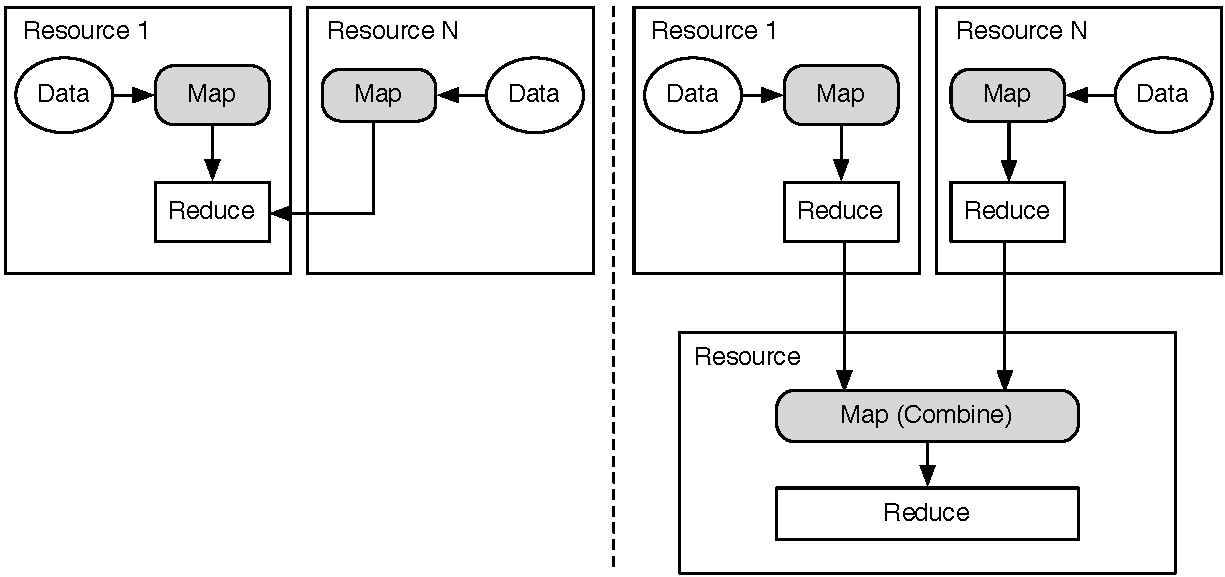
\includegraphics[width=0.48\textwidth]{figures/distributed_hierachical.pdf}
	% \label{fig:figures_distributed-mapreduce}}
%	\subfigure[Distributed PMR(implemented)]{
%		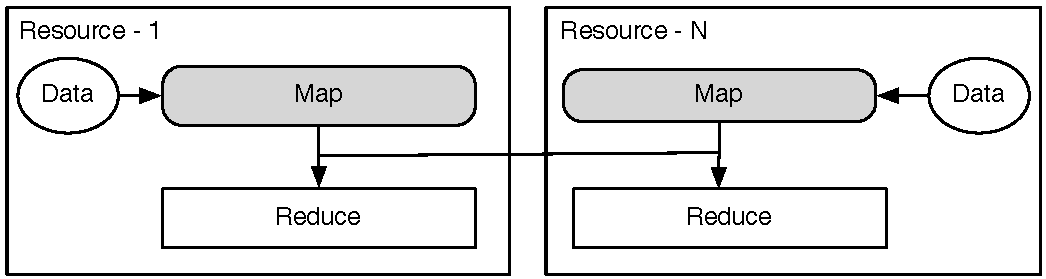
\includegraphics[width=0.4\textwidth]{figures/distributed_pmr_exchange.pdf}
%		\label{fig:figures_distributed-mapreduce-exchange}}
	% \subfigure[Hierachical PMR]{
	% 	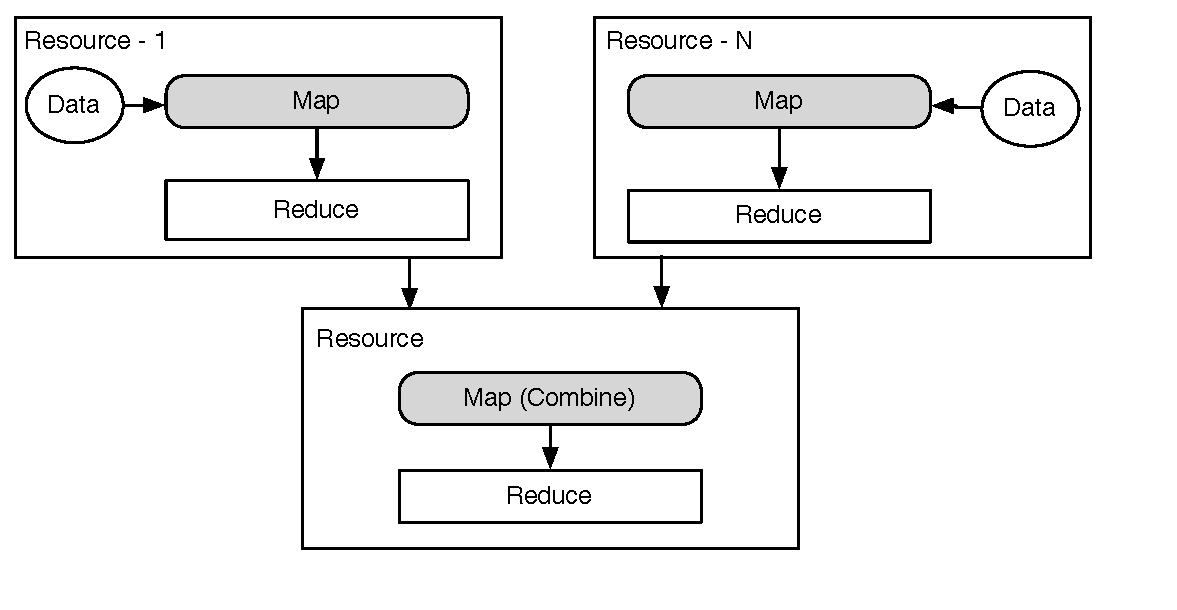
\includegraphics[width=0.4\textwidth]{figures/hierachical-mapreduce.pdf}
	%\label{fig:figures_hierachical-mapreduce}}
	\caption{\pilotmapreduce Deployment Scenarios: In the
          distributed scenario (left), the mapping tasks are run close
          to the data, the reduced tasks are then run on a single
          resource. In the hierarchical scenario (right) two complete
          MapReduce runs are
          conducted. \label{fid:distributed-mapreduce-overview}}
\end{figure}


\pilotmapreduce supports different distributed MapReduce topologies:
(i) \emph{local}, (ii) \emph{distributed} and (iii)
\emph{hierarchical}. A local PMR performs all map and reduce
computations on a single resource.
Figure~\ref{fid:distributed-mapreduce-overview} shows options (ii) and
(iii): A distributed PMR utilizes multiple resources often to run map
tasks close to the data to avoid costly data transfers; the
intermediate data is then moved to another resource for running the
reduce tasks. BigJob and BigData are used for managing CUs and DUs and
the necessary data movements. In contrast, in a hierarchical PMR the
outputs of the first complete MapReduce run are moved to a central
aggregation resource. A complete MapReduce run is then executed on
this resource to combine the results. % \jhanote{What about
%   Hierarchical: it can be distributed and/or local. Shouldnt
%   specify/discuss explicitly that it is not orthogonal to first two?}
% \alnote{for readability, I would then rather not refer to local at all
%   in this section. Also, while a local hierarchical MR is possible, it
%   doesn't really make sense, because the whole point is to reduce data
%   movement between resources. In a single cluster data needs to get
%   moved anyways.}


The Pilot-API provides a consistent API for managing both compute units (i.\,e.\ 
map and reduce tasks) and data units. Using descriptive affinities label the  
data flow between CUs, i.\,e.\ the transfer of the intermediate data, can be 
efficiently managed. Using this capability PMR can be easily scaled out to 
multiple resources to support e.\,g.\ scenario (ii) and (iii). 


% A {\it distributed-PMR} provides an opportunity to utilize multiple distributed production infrastructure to run the map and reduce computations.
% Therefore, the challenge to make use of multiple clusters to act collaboratively as one is addressed by distributed-PMR.

\alnote{\textbf{place somewhere:} Unfortunately, users cannot directly deploy a MapReduce framework such as Hadoop
on top of distributed production infrastructures to form a single larger
MapReduce cluster. Typically the internal nodes of a cluster are not directly
reachable from outside. However, MapReduce requires the master node to directly
communicate with any slave node, which is also one of the reasons why MapReduce
frameworks are usually deployed within a single cluster. [hierarchical mapreduce
paper]. Hadoop is mainly designed for cluster/local environment, but not for a
high degree of distribution.}



% FROM Pradeep: should be covered in this section resp. perf section so # fare
% In ~\cite{weissman-mr-11}, different workload data aggregation schemes are
% evaluated. High Aggregation: The MapReduce output is multiple orders of
% magnitude smaller than the input, e.g. Wordcount on English plain-text. Zero
% Aggregation: The MapReduce output is the same size as the input, e.g. the Sort
% workload. There is no MapReduce configuration regarding low aggregation
% schemes, where the output data is significant and between high and zero
% aggregation schemes. In this experiment, we try to prove that \pilotmapreduce
% is a best model for low aggregation schema applications. We choose
% ~\cite{weissman-mr-11} DMR configuration and compare it with \pilotmapreduce
% with genome sequence application, which produces significant amount of output
% and neither high aggreation nor zero aggregation. We ran experiments with
% 20GB, 40GB and 80GB on two machines and 30GB, 60GB , 120GB on 3 machines.

\section{Experiments and Results}
\label{sec-experiments}


In this section we analyze the performance and scalability of  \pilotmapreduce and compare it to Hadoop MapReduce using different applications.
For this purpose we run several experiments on FutureGrid~\cite{fg}. We run the
experiment on the FG resources: India, Sierra and Hotel. Each experiment is
repeated at least three times. For our Hadoop experiments, we use Hadoop 0.20.2. At the begin of each run a 
Hadoop cluster is started via the Torque resource management system on a
specified number of nodes. The first assigned node is used as master node
running the Hadoop JobTracker and the NameNode. The HDFS replication factor is 
set to 2 and number of reduces to 8.

\subsection{MapReduce-Based Applications}

MapReduce has been utilized in various science applications. A key performance 
factor is the amount of data that must be moved through the MapReduce system. 
The degree of data aggregation of the map tasks is thus, an important 
characteristic of a MapReduce application~\cite{weissman-mr-11}.

MapReduce application can be classified with respect to different
criteria: (i) the volume of the intermediate data (i.\,e.\ the size of
the output of the map tasks), and (ii) the volume of the output data,
(i.\,e.\ the size of reduce phase output), and the relative proportion
of these data volume. In the following we investigate two application
scenarios: WordCount and a Genome Sequencing application.

% \jhanote{The following paragraph should move to next section. Also
%   need to explain the different axes of analysis: high vs low
%   aggregation between phases; local versus distributed; hierarchical
%   versus non-hierarchical. Currently all clobbered together and
%   difficult to read} 
% \alnote{\textbf{Incorporate:} }

% Computing widely distributed data using a traditional single cluster-MapReduce
% may not achieve an optimal MapReduce runtime. Several MapReduce configurations were
% proposed for distributed data processing based on the data
% aggregation~\cite{weissman-mr-11}. In high-data aggregation application the
% MapReduce output is multiple orders of magnitude smaller than input.
% Hierarchical MapReduce configuration is considered as an optimal choice since it
% involves less amount of output data to be transferred to the combine MapReduce
% phase. In zero or ballooning data aggregation applications, the intermediate and
% output data generated is larger than or equal to input data.  So, the all the input data from
% multiple clusters is moved to a single cluster, and then MapReduce job is performed, which is 
% known as Local MapReduce. Even though the initial data transfers are costly in case of Local-MapReduce \jhanote{this
% is a term; please define a term before using it}, they are needed
% because of lack of an abstraction which manages the relationships between the
% data and compute units effectively across wide-area systems. So, BigData optimizes runtime of \pilotmapreduce by allowing
% flexibility to specify intermediate data and reduce compute affinities, and required concurrent data movement between machines and data units.

\subsubsection*{Word Count}

The Word Count application is the basis for many machine learning use cases, 
used e.\,g.\ for the classification of documents or clustering. Word Count 
generates a large volume of intermediate data ($\sim$200$\%$). The volume of the 
output data depends on the type of input data, e.\,g.\ the size of the output data is 
larger for a random input than for an input in a natural language. 


\subsubsection*{Genome Sequencing (GS)}

High-throughput genome sequencing techniques provided by Next Generation
Sequencing (NGS) platforms are changing biological sciences and biomedical
research. The data volumes generated by sequencing machines is increasing
rapidly. The distributed processing of this data requires a sophisticated
infrastructure. For this purpose, we utilize MapReduce to model an important
part of the sequencing workflow i.e, the read alignment and the duplicate
removal. We use two implementations of the workflow: the Hadoop-based 
SEQAL~\cite{seal-2011} application and a custom implementation of this workflow 
GS/PMR. Both application implement the read alignment in the mapping phase of 
the application using BWA aligner~\cite{Li:2010:FAL:1741823.1741825}. In the 
SEQAL case the duplicate removal in the reduce phase is implemented using  
Picard's rmdup~\cite{picard}. The GS/PMR reduce phase is not an exact implementation of
SEQAL's Picard rmdup implementation.We developed a custom script in python
which is based on duplicate removal description provided in ~\cite{seal-2011}. 
The GS/PMR reducer removes duplicate reads based on the key fields-chromosome,
position, strand of GS/PMR mapper output.

%%%%%%%%%%%%%%%%%%%%%%%%%%%%%%%%%%%%%%%%%%%%%%%%%%%%%%%%%%%%%%%%%%%%%%%%%%%%

\subsection{Characterizing Word Count}
\alnote{random vs. non-random data}

In the first experiment, we benchmark the performance of \pilotmapreduce and
Hadoop using a simple Word Count application on a single resource. For both
frameworks, a total of 8 nodes on India machine are used. In all scenarios the
input data is pre-staged on the respective resources, i.\,e.\ for Hadoop the
data is located in the HDFS file system, for PMR the data is stored on a shared
file system. We set the total number of reduces to 8 for both Hadoop and
\pilotmapreduce; further, the default chunk size of 128\,MB is used. A HDFS
replication factor of 2 is used.

The runtime of local PMR include time to chunk input data, running the mapping
CUs, shuffling (which again comprises of sorting and the intermediate data
transfer, and finally running the reduce CUs.
Figure~\ref{fig:figures_wc_pmr_hmr} shows the results. The runtime
of Hadoop MapReduce include time to load input source data into HDFS and
MapReduce runtime.

\begin{figure}[ht]
	\centering
		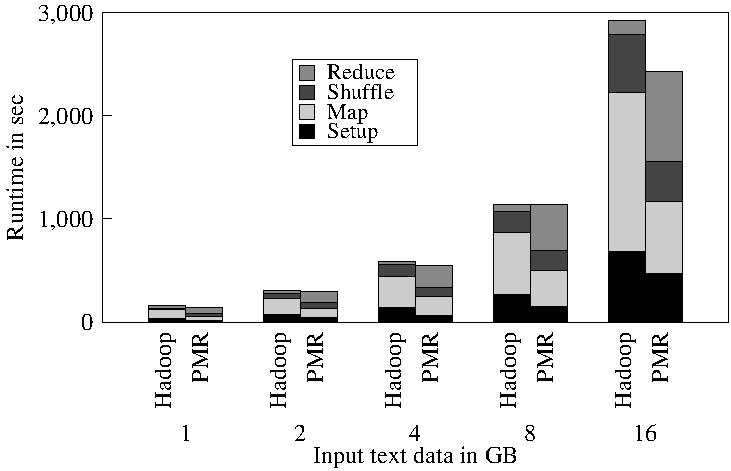
\includegraphics[width=0.47\textwidth]{figures/wc_pmr_hmr.pdf}
\caption{Word Count: PMR versus Hadoop MapReduce(HMR): The performance of Hadoop and PMR is 
comparable. The runtime increase with the input data size. Hadoop tasks have a 
notable higher startup time than PMR tasks.} 	
\label{fig:figures_wc_pmr_hmr}
\end{figure}		
	
The performance of both Hadoop and PMR is comparable. The time to solution 
increased linearly as data size increased for all cases. In particular for 
larger volumes of input data PMR shows a better performance than Hadoop. 
Further, the results indicate that the shuffle phase is critical in particular 
if larger volumes of data need to be sorted and moved as in the Word Count 
application where the intermediate data is about 200\,\% of the input data.


% The total runtime increased linearly as data size increased for both the MapReduces. Hadoop is optimized and performs well with shared file systems.

% greater than Map phase time of Local-PMR because Hadoop MR involves preparing input splits and starting the map tasks, whereas in Pilot MapReduce, chunk time is considered seperatly and Map phase involves submitting of map compute units. The chunking time of distributed-Pilot MapReduce is less when compared to Local-PMR, since the data is halved and distributed to two machines. \pnote{ Andre::question::Hadoop uses logical splitting of files, where as PMR chunks the files physically, wiritng to disk, this is a performance bottlneck. Is acessing a single file, by many parallel subjobs cause problems?}. The shuffle phase is considered only in Hadoop MapReduce, where as the exchange is involved in Pilot MapReduce. The input to the reduce phase in all the three MapReduce increased linearly with input data. In local-PMR is < 1sec as the data is moved within cluster using SAGA file adaptor. In distributed PMR, the time to exchange data between India and Hotel also increased linearly with input data size. The Reduce phase is high for Pilot MR since the reduce compute units has to read intermediate data from the disk and write output data to the disk, where as in Hadoop MapReduce reduce phase, the intermediate data is available in memory and write the output to HDFS.



\alnote{Not sure whether we should mention these - these issues are well-known: Observed performance issues:
1) HDFS performs better when nodes local data directory is used.. But performance degrades if shared storage is used. 			
2) when a single node is used to launch all workers, hadoop fails with lot of memory problems, whereas PMR successfully completed all tasks.			
reasons for this problem}

%http://tech.backtype.com/the-dark-side-of-hadoop+J204		

\subsection{Characterizing Genome Sequencing}

In this section, we compare and contrast GS/PMR and SEQAL. For both
applications, we utilize the same set of input data comprising of different
sizes of read files and the reference genome. SEQAL, however, expects the input
data in a different format (prq instead of fastq); thus, the data was previously
converted to meet the SEQAL requirements. For PMR, the fastq files from
sequencing machines are directly used; further, a custom chunk script is used to
chunk the fastq files based on the number of reads. We make sure that the chunk
size for both SEQAL and PMR is equal. For both frameworks, a total of 4 nodes on
FutureGrid sierra machine, 8 reduces, 2 workers/node, default chunk size of
128\,MB is used. For Hadoop based SEQAL, the replication factor of two is used.
Since SEQAL and GS/PMR utilize different duplicate removal tools in the reduce
phase, we focus our investigation on the map phase.

%  to compare scalability of PMR across clusters, we are
% interested in only in the execution of map phase. SEQAL provides an option to
% turnoff the reduce phase and just perform the map phase. For PMR a custom 
% mapper
% script is developed in Python, which uses core BWA aligner. 

\begin{figure}[ht]
	\centering
		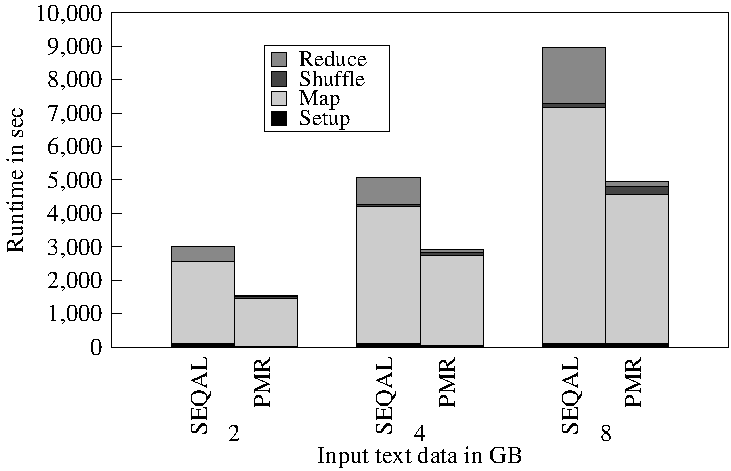
\includegraphics[width=0.47\textwidth]{figures/gs_seq_pmr.pdf}
\caption{SEQAL and GS/PMR: GS/PMR provides a marginal better performance that 
SEQAL. The overhead of SEQAL is mainly attributed to the used HDFS configuration 
using a shared file system.} 	
\label{fig:gs_seq_pmr}
\end{figure}		

Figure~\ref{fig:gs_seq_pmr} shows the results of both applications. In the
setup time of SEQAL, Hadoop copies the reference genome archive to all the 
nodes and extracts it so it is available locally.
In comparison to Word Count both GS application are more compute intensive,
i.\,e.\ the ratio between computation in the map phase and the size of the input
data is significant larger. Notably, SEQAL requires a longer time-to-completion
than GS/PMR. This is mainly caused by a non-optimal configuration of Hadoop: The
local disks available on FG is too small for the used input data; thus, HDFS had
to be configured to utilize a shared, distributed file system, which leads to a
non-optimal performance during the I/O intensive map phase. The difference in
the reduce phase mainly originate from the different implementations of the
duplicate removal process in SEQAL and GS/PMR. 

\alnote{Pradeep: Please elaborate a bit on the differences}

\subsection{Distributed MapReduce}

In this section, we evaluate the performance and scalability of (i) a 
distributed and (ii) hierarchical \pilotmapreduce configuration (see
section~\ref{sec:pmr-distributed}) using the Word Count application on natural 
language and on random data as well as the genome sequencing application. In the 
distributed scenario (i) \pilotmapreduce map CUs are distributed across 
two machines, in the  hierarchical scenario (ii) an additional MapReduce run is 
necessary for combining and aggregating the data.

For Word Count we compare a distributed and hierarchical PMR configuration with
the performance of a single resource Hadoop configuration. We utilize two
machines, Sierra and Hotel, and assume that the initial input 16GB data is equally
distributed on these two machines. That means that for the Hadoop scenario half 
of the input data is moved from Sierra to Hotel prior to running the actual 
MapReduce job. Unfortunately, the FutureGrid firewall rules prohibited the usage 
of a distributed Hadoop setup. For all configurations, we use a total of 8 
nodes. 

\alnote{Add hierarchical MR}
Figure~\ref{fig:allmrs_rands} shows the results. In general, the distributed 
PMR performs better than Hadoop mainly due to the time necessary to move the 
input files to the single Hadoop resource. However, the map and reduce phase 
runtime of PMR are much longer than in the Hadoop case. This is mainly caused by 
the resource heterogeneity and the resulting scheduling overhead: the slowest node determines the overall runtime of both the map and reduce phase.


For Word Count on random data, distributed PMR performs better than other
implementations since it moves only required data in the intermediate phase and
there are no initial or combine outputs overhead. The intermediate data that
needs to be moved from Sierra to Hotel is 15.45\,GB, and data related to each
reduce nearly 1.9GB is segregated as data unit. The Pilot-Data supports parallel
transfer of data units, which results in an effective data transfer of 1.9GB
This leads to the performance of distributed PMR. Hadoop suffers the initial
data transfer of 8GB from Sierra to Hotel and HDFS load times. In hierarchical
Hadoop, we transferred the total output reduce data 14.8GB using Pilot-Data,
where each data unit consists a reduce output file. So that all reduces can be
transferred in parallel and effective data transfer would be nearly 1.85GB. But
loading 14.8GB on Hotel contributed significantly towards its the entire
runtime. Hierarchical PMR is closer to distributed PMR, but it involves combine
MapReduce overhead.

For Word Count on natural language text data, Both hierarchical Hadoop and PMR
performs better than other implementations, since they involves very less amount
of output data generated and involves less combine overhead. Hadoop suffers the
initial data transfer of 8GB from Sierra to Hotel and HDFS load times. In case
of distributed PMR the intermediate data 12.85\,GB moved using Pilot-Data
resulting in a effective data transfer of 1.6\,GB. The data transfer and amount
to reduce the entire intermediate data results in higher runtime of distributed
PMR.


\pnote{observed when running distributed PMR; Still need to be modified, But 
checking in as time is up..}


\begin{figure}[ht]
	\centering
		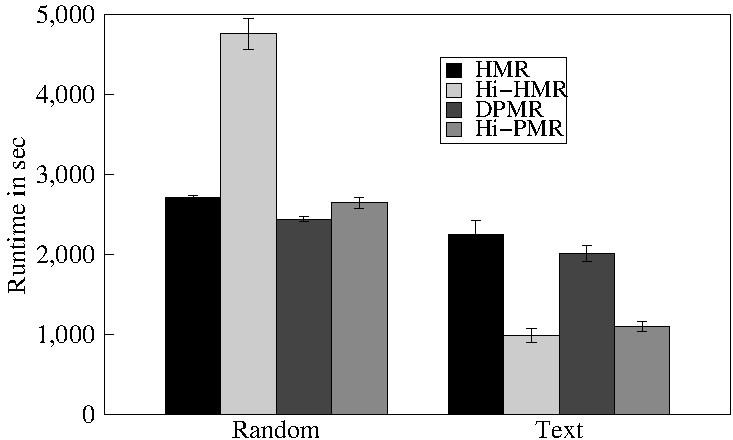
\includegraphics[width=0.47\textwidth]{figures/allmrs_rands.pdf}
\caption{Word Count Using Hadoop MapReduce(HMR), Hierarchical HMR (Hi-HMR), Distributed PMR(DPMR) and 	Hierarchical PMR (Hi-PMR)} 	
\alnote{only show 16 GB case for Hadoop, hierarchical Hadoop, DPMR and HPMR. Two clusters of bars for random and non-random data}
\label{fig:allmrs_rands}
\end{figure}		


For the genome sequencing we utilize India and Hotel and a total of 32 nodes.
\alnote{in 5.3 we only use 4 nodes? Why that?} For both distributed and
hierarchical PMR, Hotel is used for running the reduce tasks respectively the
combining MR run. This setup ensures that the necessary data transfers are
minimized.

% % \pnote{Weissmanns paper doesn't talk about low workload scheme applications
% where reduce output is still significantly large.. ( it talks about zero,
% high, balooning ).. so we have a model for these type of applications. why
% weissmanns DMR is choosed?? LMR involves huge amount of initial data transfer.
% GMR need global filesystem across clusters, which is difficult to have, and
% latencies issues in moving files. So, DMR is a potential choice over LMR and
% GMR.}


\begin{figure}[ht]
	\centering
		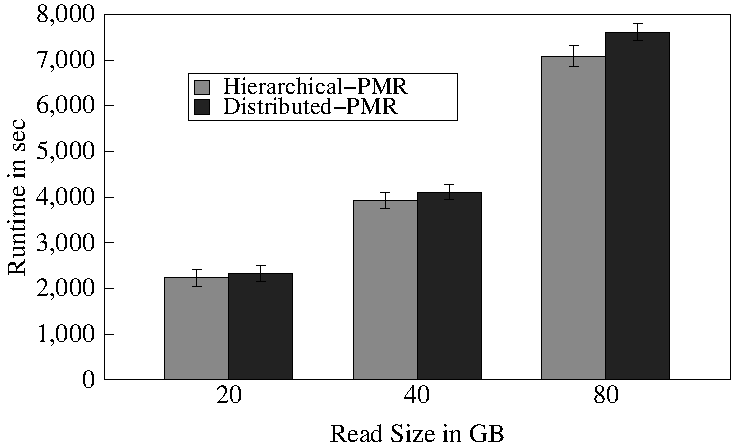
\includegraphics[width=0.47\textwidth]{figures/gs_hihmr_dpmr.pdf}
\caption{GS/PMR Using Hierarchical PMR(Hi-PMR) vs. Distributed PMR(DPMR)} 	
\label{fig:gs_hihmr_dpmr}
\end{figure}		


The runtime of the hierarchical PMR is lesser than in the distributed case because of low data need to be transferred and less overhead in combine MapReduce phase. The data movement
for both hierarchical and distributed PMRs is shown in table ~\ref{tab:data-volumes-gs}

\alnote{What is transferred from where to where? In the experiments data is always moved from sierra to hotel, because of higher data transfer rates and hotel is fastest machine}
\begin{table}[h]
\begin{tabular}{|l|c|c|c|}
\hline
\textbf{Application} &\textbf{Input} &\textbf{Intermediate} &\textbf{Output}\\
\hline
GS/PMR 		&20\,GB &18.65\,GB		 &6.2\,GB\\
\hline
Word Count (English) &16\,GB&29.47\,GB&20\,MB\\
\hline
Word Count (random) &16\,GB&29.6\,GB&29.5\,GB\\
\hline
\end{tabular}
\caption{Data Volumes for different Application Scenarios}
\label{tab:data-volumes}
\alnote{Pradeep: please fill out}
\end{table}


\alnote{What is transferred from where to where?}
\begin{table}[h]
\begin{tabular}{|l|c|c|c|c|}
\hline
\textbf{MapReduce} &\textbf{Data to be moved} &\textbf{Effective 
data transfer}&\textbf{Parallel transfers}\\
\hline
HMR  &8\,GB &8\,GB		 &1\\
\hline
Hi-HMR &14.8\,GB&1.85\,GB&8\\
\hline
DPMR&15.45\,GB&1.93\,GB&8\\
\hline
Hi-PMR&15.20\,GB&1.9\,GB&8\\
\hline
\end{tabular}
\caption{Data Volumes for Word Count application with 16GB random data}
\label{tab:data-volumes-random}
\alnote{Pradeep: please fill out}
\end{table}


\alnote{What is transferred from where to where?}
\begin{table}[h]
\begin{tabular}{|l|c|c|c|c|}
\hline
\textbf{MapReduce} &\textbf{Data to be moved} &\textbf{Effective 
data movement}&\textbf{Parallel transfers}\\
\hline
HMR  &8\,GB &8\,GB		 &1\\
\hline
Hi-HMR &16\,MB&2\,MB&8\\
\hline
DPMR&12.85\,GB&1.6\,GB&8\\
\hline
Hi-PMR&16\,MB&2\,MB&8\\
\hline
\end{tabular}
\caption{Data Volumes for Word Count application with 16GB natural langauge text data}
\label{tab:data-volumes-text}
\alnote{Pradeep: please fill out}
\end{table}

\begin{table*}[h]
\begin{tabular}{|l|c|c|c|c|}
\hline
\textbf{MapReduce} &\textbf{Read size} &\textbf{Data to be moved} &\textbf{Effective 
data transfer}&\textbf{Parallel transfers}\\
\hline
Hi-HMR &20\,GB&3.04\,GB&0.38\,GB&8\\
\hline
DPMR &20\,GB&9.32\,GB&1.22\,GB&8\\
\hline

\hline
Hi-HMR &40\,GB&5.79\,GB&0.724\,GB&8\\
\hline
DPMR &40\,GB&18.46\,GB&2.42\,GB&8\\
\hline

\hline
Hi-HMR &80\,GB&8.73\,GB&1.09\,GB&8\\
\hline
DPMR &80\,GB&35.6\,GB&\,4.45GB&8\\
\hline

\end{tabular}
\caption{Data Volumes for Genome Sequencing application}
\label{tab:data-volumes-gs}
\alnote{Pradeep: please fill out}
\end{table*}



% A correlation exists between the input data sizes and the performance of
% MapReduce configurations. 

\alnote{The following paragraph needs refinement}
Figure~\ref{fig:gs_hihmr_dpmr} shows the results. In both scenarios the runtime
increases with the input data size. In scenario (i), the increase in runtime is
due to the amount of data, to be processed by map phase, moved in the shuffle
phase and processed by reduce phase. In scenario (ii), the higher runtime is
mainly due to the additional map and reduce runs that are necessary While the
amount of data that needs to be moved in both scenarios is comparable (see
table~\ref{tab:data-volumes}), a current limitation of the hierarchical PMR
implementation is the lack of a parallel file transfer between the MapReduce
jobs. In summary, the hierarchical PMR outperforms the distributed PMR if output
of the reduce phase is much lower than the intermediate data that would have
been required to transfer otherwise.



% Analysis
Running MapReduce on widely distributed data using a single resource
configuration may not yield into an optimal runtime. Depending on the
application's characteristics a distributed or hierarchical deployment may show
a better performance. In high aggregation applications, such as the genome 
sequencing application, the MapReduce output is multiple orders of magnitude 
smaller than input. A hierarchical MapReduce configuration is considered a good 
choice for such a scenario since it involves less amount of output data that 
needs to be transferred. In no data aggregation applications, i.\,e.\ the 
output data generated is larger than or equal to input data, a distributed 
configuration is better suited. 


In summary, PMR provides the flexibility to deploy MapReduce workload in
different configurations optimizing the performance with respect to the
characteristics of different application workloads: a hierarchical setup is good
for applications with highly aggregated output data as GS/PMR, while a normal
distributed setup is good for application with a highly aggregate intermediate
output. A major limitation of Hadoop is still its inflexibility with respect to
supporting different kind of resources and topologies. In our case e.\,g.\ we
were not able to run Hadoop across more than two machines on FG due to firewall
issues.


\note{Points to make:
\begin{itemize}
	\item PMR is flexible and extensible
	\item different workloads require different configurations
	\item Hadoop is difficult to setup to spawn multiple resources
	\item hierarchical PMR is good for high-aggregation workloads
\end{itemize}}




\note{
PMR tts = max( map  on india, map on  sierrra, map on hotel) + max( exchange of 
intermediate data between all machines(n) ( r * n-1 concurrent exchanges)) + max 
( reduce phase on  india, reduce on  sierrra, reduce on hotel)
--- experiments done for local PMR on each individual cluster.. once time 
taken to transfer intermediate data between machines is obtained.. then tts 
for PMR can be calculated and compared to HPMR.
}

\alnote{\textbf{For Analysis:}
In distributed-PMR on m clusters
with n reduces distributed evenly across clusters involve n*(m-1) parallel data
transfers to complete the intermediate data movement. Thus BigData play a major
role in reducing the runtime of a distributed-PMR running on multiple clusters.
}

\section{Discussion and Future Work}
\label{sec-conclusion}

\pilotmapreduce provides a flexible runtime environment for running
MapReduce applications on general-purpose distributed infrastructures,
such as XSEDE and FutureGrid. In contrast to Hadoop, previous setup of
clusters (including Hadoop/HDFS) and various other daemons is not
required. Pilot-MapReduce provides flexibility and extensible building
block, which allows the flexible usage of sorting in the shuffle, more
fine-grained control of data localities and transferred as well as
support for different MapReduce topologies. Using these capabilities,
applications with different characteristics, e.\,g.\ compute/IO and
data aggregation ratios, can be efficiently supported.

%Pilot-Abstractions and affinities are a powerful tool

In the future we will extend the capabilities of BigData to support
use cases such as data streaming, data caching as well as different
data/compute scheduling heuristics. Further, we will explore scenarios
and applications with dynamic data and execution.  An obvious and
trivial extension will be to implement Iterative MapReduce using PMR.
A clear advantage will be to obviate the need to distinguish between
static and dynamic data, for PMR will be able to treat both
symmetrically.


% The following two commands are all you need in the
% initial runs of your .tex file to
% produce the bibliography for the citations in your paper.
\bibliographystyle{abbrv}
%\bibliographystyle{unsrt}
\bibliography{pilotjob,saga,saga-related,mrbib}  % sigproc.bib is the name of the Bibliography in this case
% You must have a proper ".bib" file
%  and remember to run:
% latex bibtex latex latex
% to resolve all references
%
% ACM needs 'a single self-contained file'!
%


\subsection*{Acknowledgments}
\scriptsize This work is funded by NSF CHE-1125332 (Cyber-enabled
Discovery and Innovation), HPCOPS NSF-OCI 0710874 award, NSF-ExTENCI
(OCI-1007115) and NIH Grant Number P20RR016456 from the NIH National
Center For Research Resources. Important funding for SAGA has been
provided by the UK EPSRC grant number GR/D0766171/1 (via OMII-UK) and
the Cybertools project (PI Jha) NS-F/LEQSF (2007-10)-CyberRII-01. SJ
acknowledges the e-Science Institute, Edinburgh for supporting the
research theme. Distributed Programming Abstractions \& 3DPAS. SJ ac-
knowledges useful related discussions with Jon Weissman (Minnesota)
and Dan Katz (Chicago). We thank J Kim (CCT) for assistance with
genome sequencing application. This work has also been made possible
thanks to computer resources provided by TeraGrid TRAC award
TG-MCB090174 (Jha). This document was developed with support from the
US NSF under Grant No. 0910812 to Indiana University for FutureGrid:
An Experimental, High-Performance Grid Test-bed.
\end{document}
